% !TeX root=../journalDeepMedic.tex


%%%%%%%%%%%%%%%%%%%%%%%%%%%%%%%%%%%%%%%%%%%%%%%%%%%%%%%%%%%%%%
%%%%%%%%%%%%%%%%%%%% EVALUATION %%%%%%%%%%%%%%%%%%%%%%%%%%%%%%
%%%%%%%%%%%%%%%%%%%%%%%%%%%%%%%%%%%%%%%%%%%%%%%%%%%%%%%%%%%%%%

\section{Evaluation on Clinical Data}
\label{sec:evaluation}

The proposed system consisting of the DeepMedic CNN architecture, optionally coupled with a fully connected CRF, is evaluated on three lesion segmentation tasks including challenging clinical data from patients with traumatic brain injuries, brain tumors, and ischemic stroke. Quantitative evaluation and comparisons with state-of-the-art are reported for each of the tasks.

\subsection{Traumatic Brain Injuries}
\label{subsec:evalTbi}

\subsubsection{Material and Pre-Processing}
\label{subsubsec:materialTbi}

Sixty-six patients  with moderate-to-severe TBI who required admission to the Neurosciences Critical Care Unit at Addenbrooke's Hospital, Cambridge, UK, underwent imaging using a 3-Tesla Siemens Magnetom TIM Trio within the first week of injury. Ethical approval was obtained from the Local Research Ethics Committee (LREC 97/290) and written assent via consultee agreement was obtained for all patients. The structural MRI sequences that are used in this work are isotropic MPRAGE (1$mm\times$1$mm\times$1$mm$), axial FLAIR, T2 and Proton Density (PD) (0.7$mm\times$0.7$mm\times$5$mm$), and Gradient-Echo (GE) (0.86$mm\times$0.86$mm\times$5$mm$). All visible lesions were manually annotated on the FLAIR and GE sequences with separate labeling for each lesion type. In nine patients the presence of hyperintense white matter lesions that were felt to be chronic in nature were also annotated. Artifacts, for example, signal loss secondary to intraparenchymal pressure probes, were also noted. For the purpose of this study we focus on binary segmentation of all abnormalities within the brain tissue. Thus, we merged all classes that correspond to intra-cerebral abnormalities into a single \quot{lesion} label. Extra-cerebral pathologies such as epidural and subdural hematoma were treated as background. We excluded two datasets because of corrupted FLAIR images\ignore{13296, 17792}, two cases because no lesions were found\ignore{13776, 15883} and one case \ignore{11976} because of a major scanning artifact corrupting the images. This results in a total of 61 cases used for quantitative evaluation. Brain masks were obtained using the ROBEX tool (\cite{Iglesias2011}). All images were resampled to an isotropic $1mm^3$ resolution, with dimensions 193$\times$229$\times$193 and affinely registered (\cite{Studholme1999}) to MNI space using the atlas by \cite{Grabner2006}. No bias field correction was used as preliminary results showed that this can negatively affect lesion appearance. Image intensities were normalized to have zero-mean and unit variance, as it has been reported that this improves CNN results (\cite{Jarrett2009}).

\subsubsection{Experimental Setting}
\label{subsubsec:tbiExperimentalSetting}

\textbf{Network configuration and training:} The network architecture corresponds to the one described in Sec.~\ref{subsec:valMultiscale}, i.e. a dual-pathway, 11-layers deep CNN. The training data is augmented by adding images reflected along the sagittal axis. To make the network invariant to absolute intensities we also shift the intensities of each MR channel $c$ of every training segment by $i_c = r_c \sigma_c$. $r_c$ is sampled for every segment from $\mathcal{N}(0,0.1)$ and $\sigma_c$ is the standard deviation of intensities under the brain mask in the corresponding image. The network is regularized using dropout (\cite{hinton2012dropout}) with a rate of 2\% on all convolutional layers, which is in addition to a 50\% rate used on the last two layers. The network is evaluated with 5-fold cross-validation on the 61 subjects.

\textbf{CRF configuration:} The parameters of the fully connected CRF are determined in a configuration experiment using random-search and 15 randomly selected subjects from the TBI database with predictions from a preliminary version of the corresponding model. The 15 subjects are reshuffled into the 5-folds used for subsequent evaluation.

\textbf{Random Forest baseline:} We have done our best to set up a competitive baseline for comparison. We employ a context-sensitive Random Forest, similar to the model presented by \cite{Zikic2012} for brain tumors except that we apply the forest to the MR images without additional tissue specific priors. We train a forest with 50 trees and maximum depth of 30. Larger size did not improve results. Training data points are approximately equally sampled from lesion and background classes, with the optimal balance empirically chosen. Two hundred randomized cross-channel box features are evaluated at each split node with maximum offsets and box sizes of 20mm. The same folds of training and test sets are used as for our CNN approach.

\subsubsection{Results}
\label{subsec:resTbi}


\begin{table}[!h]
\centering
\scriptsize
\caption{Performance of \textit{DeepMedic} and an \textit{ensemble} of three networks on the TBI database. For comparison, we provide results for a Random Forest baseline. Values correspond to the mean (and standard deviation). Numbers in bold indicate significant improvement by the CRF post-processing, according to a two-sided, paired t-test on the DSC metric (*$p<5 \cdot 10^{-2}$, **$p<10^{-4}$).}
\label{table:accuracyTbiTrio}
\begin{tabular}{@{}llllll@{}}
\toprule
\multicolumn{1}{c}{}	& DSC			& Precision		& Sensitivity		& ASSD					& Haussdorf 	\\ \midrule
R. Forest			& 51.1(20.0)		& 50.1(24.4) 	& 60.1(15.8)			& 8.29(6.76)				& 64.17(15.98)	\\
R. Forest+CRF		& \textbf{54.8(18.5)**}	& 58.6(23.1)	& 56.9(17.4)		& 6.71(5.01)				& 59.45(15.52)	\\
DeepMedic			& 62.3(16.4)		& 65.3(18.8)		& 64.4(16.3)			& 4.24(2.64)				& 56.50(15.88)	\\
DeepMedic+CRF		& \textbf{63.0(16.3)**} & 67.7(18.2)	& 63.2(16.7)		& 4.02(2.54)				& 55.68(15.93)	\\
Ensemble				& 64.2(16.2)		& 67.7(18.3)		& 65.3(16.3)			& 3.88(2.33)				& 54.38(15.45)	\\
Ensemble+CRF			& \textbf{64.5(16.3)*} 	& 69.8(17.8)		& 63.9(16.7)		& 3.72(2.29)				&52.38(16.03)	\\
\bottomrule
\end{tabular}
\end{table}


Table \ref{table:accuracyTbiTrio} summarizes the results on TBI. Our CNN significantly outperforms the Random Forest baseline, while the relatively overall low DSC values indicate the difficulty of the task.  Due to randomness during training the local minima where a network converges are different between training sessions and some errors they produce differ (\cite{Choromanska2015}). To clear the unbiased errors of the network we form an \textit{ensemble} of three similar networks, aggregating their output by averaging. This ensemble yields better performance in all metrics but also allows us to investigate the behaviour of our network focusing only on the biased errors. Fig.~\ref{fig:evalTbiAccVsVol} shows the DSC obtained by the ensemble on each subject in relation to the manually segmented and predicted lesion volume. The network is capable of segmenting cases with very small lesions, although, performance is less robust in these cases as even small errors have large influence on the DSC metric. Investigation of the predicted lesion volume, which is an important biomarker for prognostication, shows that the network is neither biased towards the lesion nor background class, with promising results even on cases with very small lesions. Furthermore, we separately evaluate the influence of the post-processing with the fully connected CRF. As shown in Table \ref{table:accuracyTbiTrio}, the CRF yields improvements over all classifiers. Effects are more prominent when the performance of the primary segmenter degrades, which shows the robustness of this regulariser. Fig.~\ref{fig:evalTbiVisualQuality} shows three representative cases.

%+210 to left and -210 to right if I want to move one subfigure.

\begin{figure}[!ht]
%\vspace{-1pt} %takes away some white space before figure
\centering
\begin{subfigure}[b]{1.0\textwidth}
	\centering
	%\includegraphics[clip=true, trim=0pt 305pt 0pt 15pt, width=1.0\textwidth]{figures/evaluationSection/tbi/resultsVsLesionVolume/tbiAccuracyJournal.pdf}
	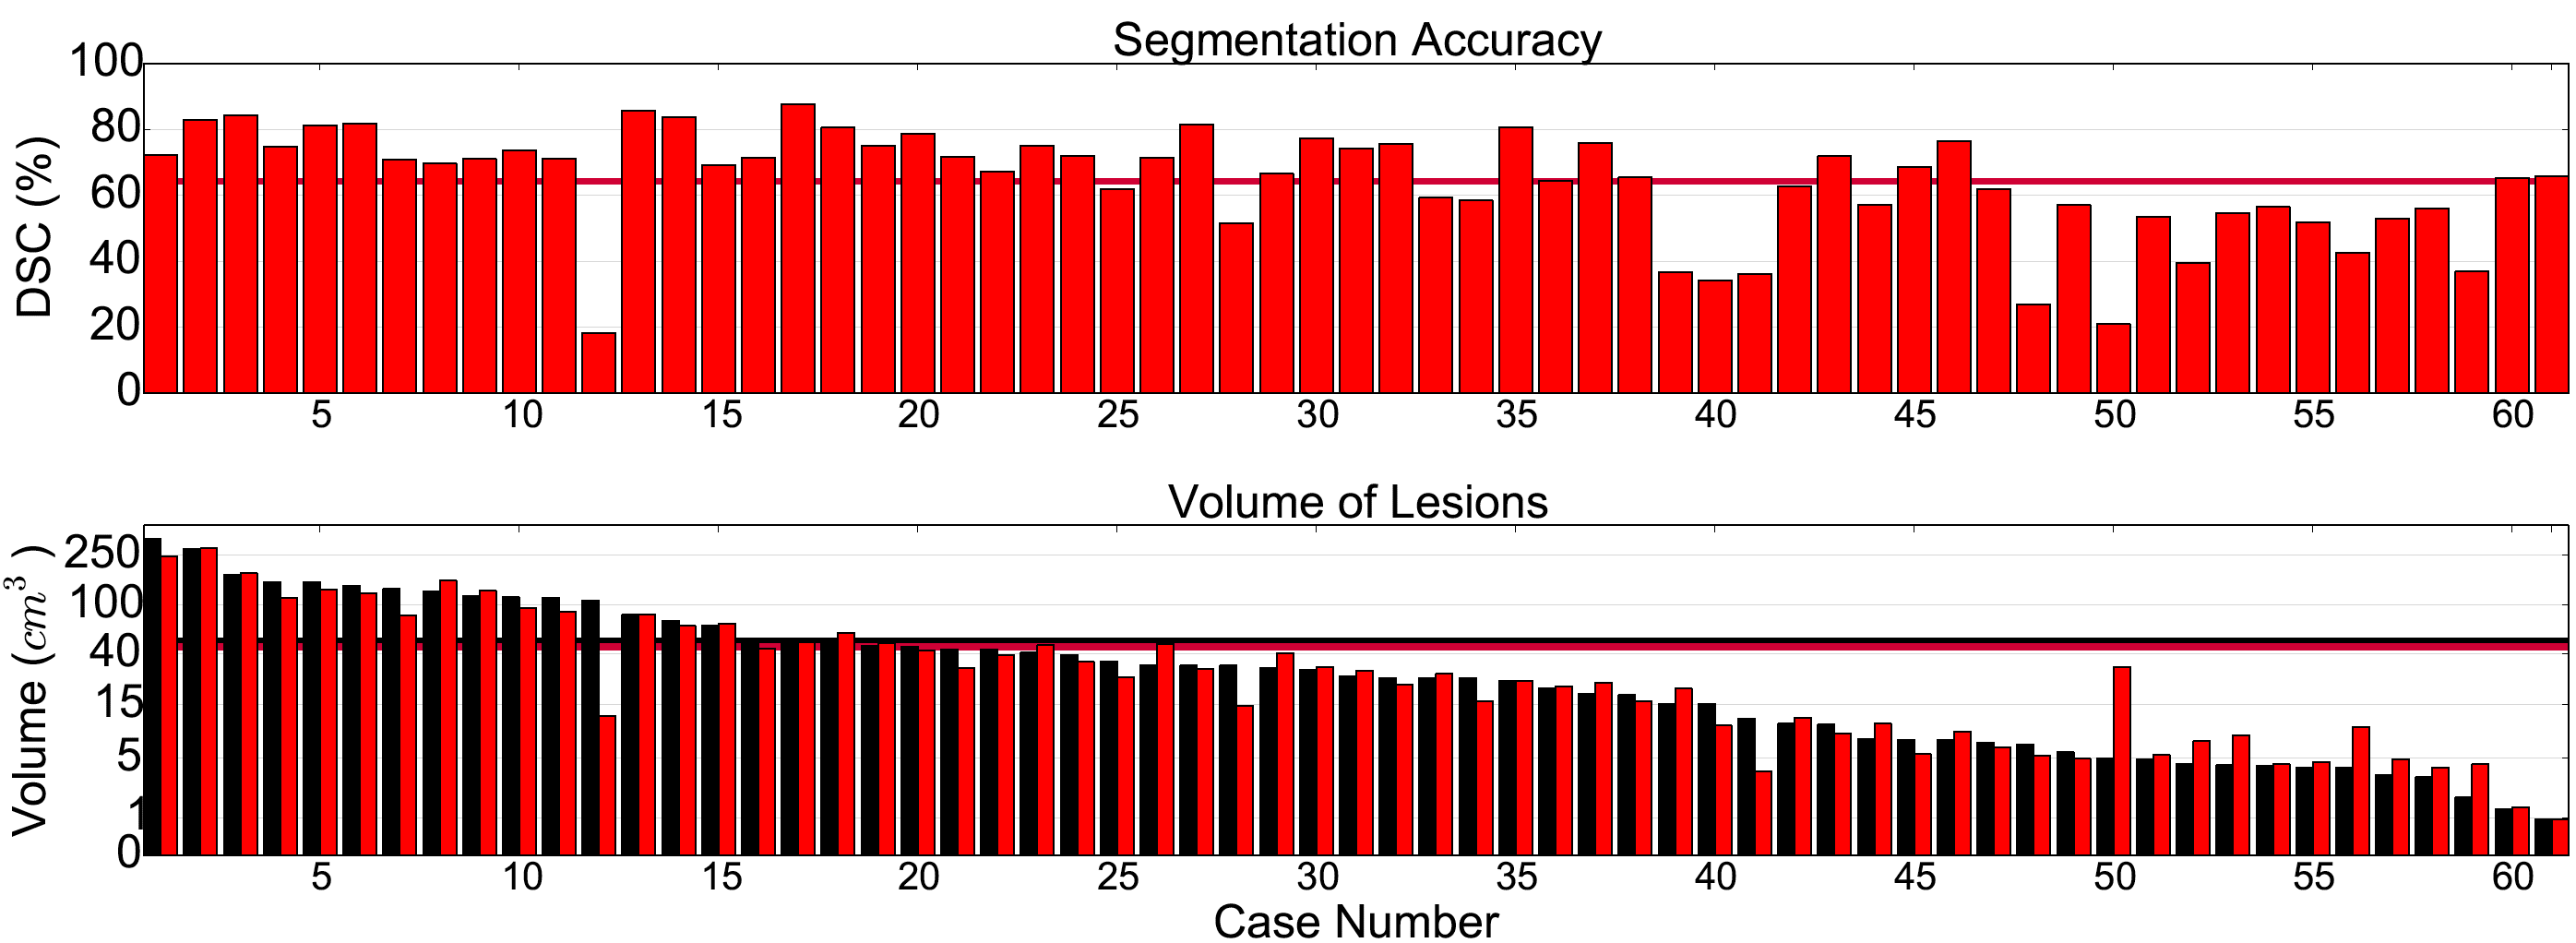
\includegraphics[clip=true, trim=0pt 0pt 0pt 0pt, width=1.0\textwidth]{figures/evaluationSection/tbi/resultsVsLesionVolume/tbiAccuracyJournal_nonReg.png}
\end{subfigure}
\vspace{-0pt} %takes away some white space before the caption
\caption{(Top) DSC achieved by our ensemble of three networks on each of the 61 TBI datasets. (Bottom) Manually segmented (black) and predicted lesion volumes (red). Note here the logarithmic scale. Continuous lines represent mean values. The outlying subject 12 presents small TBI lesions, which are successfully segmented, but also vascular ischemia. Because it is the only case in the database with the latter pathology, the networks fail to segment it as such lesion was not seen during training.}
\label{fig:evalTbiAccVsVol}
\vspace{-10pt}
\end{figure}
%\vspace{-1pt} %takes away some white space before figure

\begin{figure}[!ht]
%\vspace{-1pt} %takes away some white space before figure
\centering
\begin{subfigure}[b]{1.0\textwidth}
	\centering
	%\includegraphics[clip=true, trim=0pt 240pt 0pt 0pt, width=1.0\textwidth]{figures/evaluationSection/tbi/visualsQualitatively/visualsQualitatively3.png}
	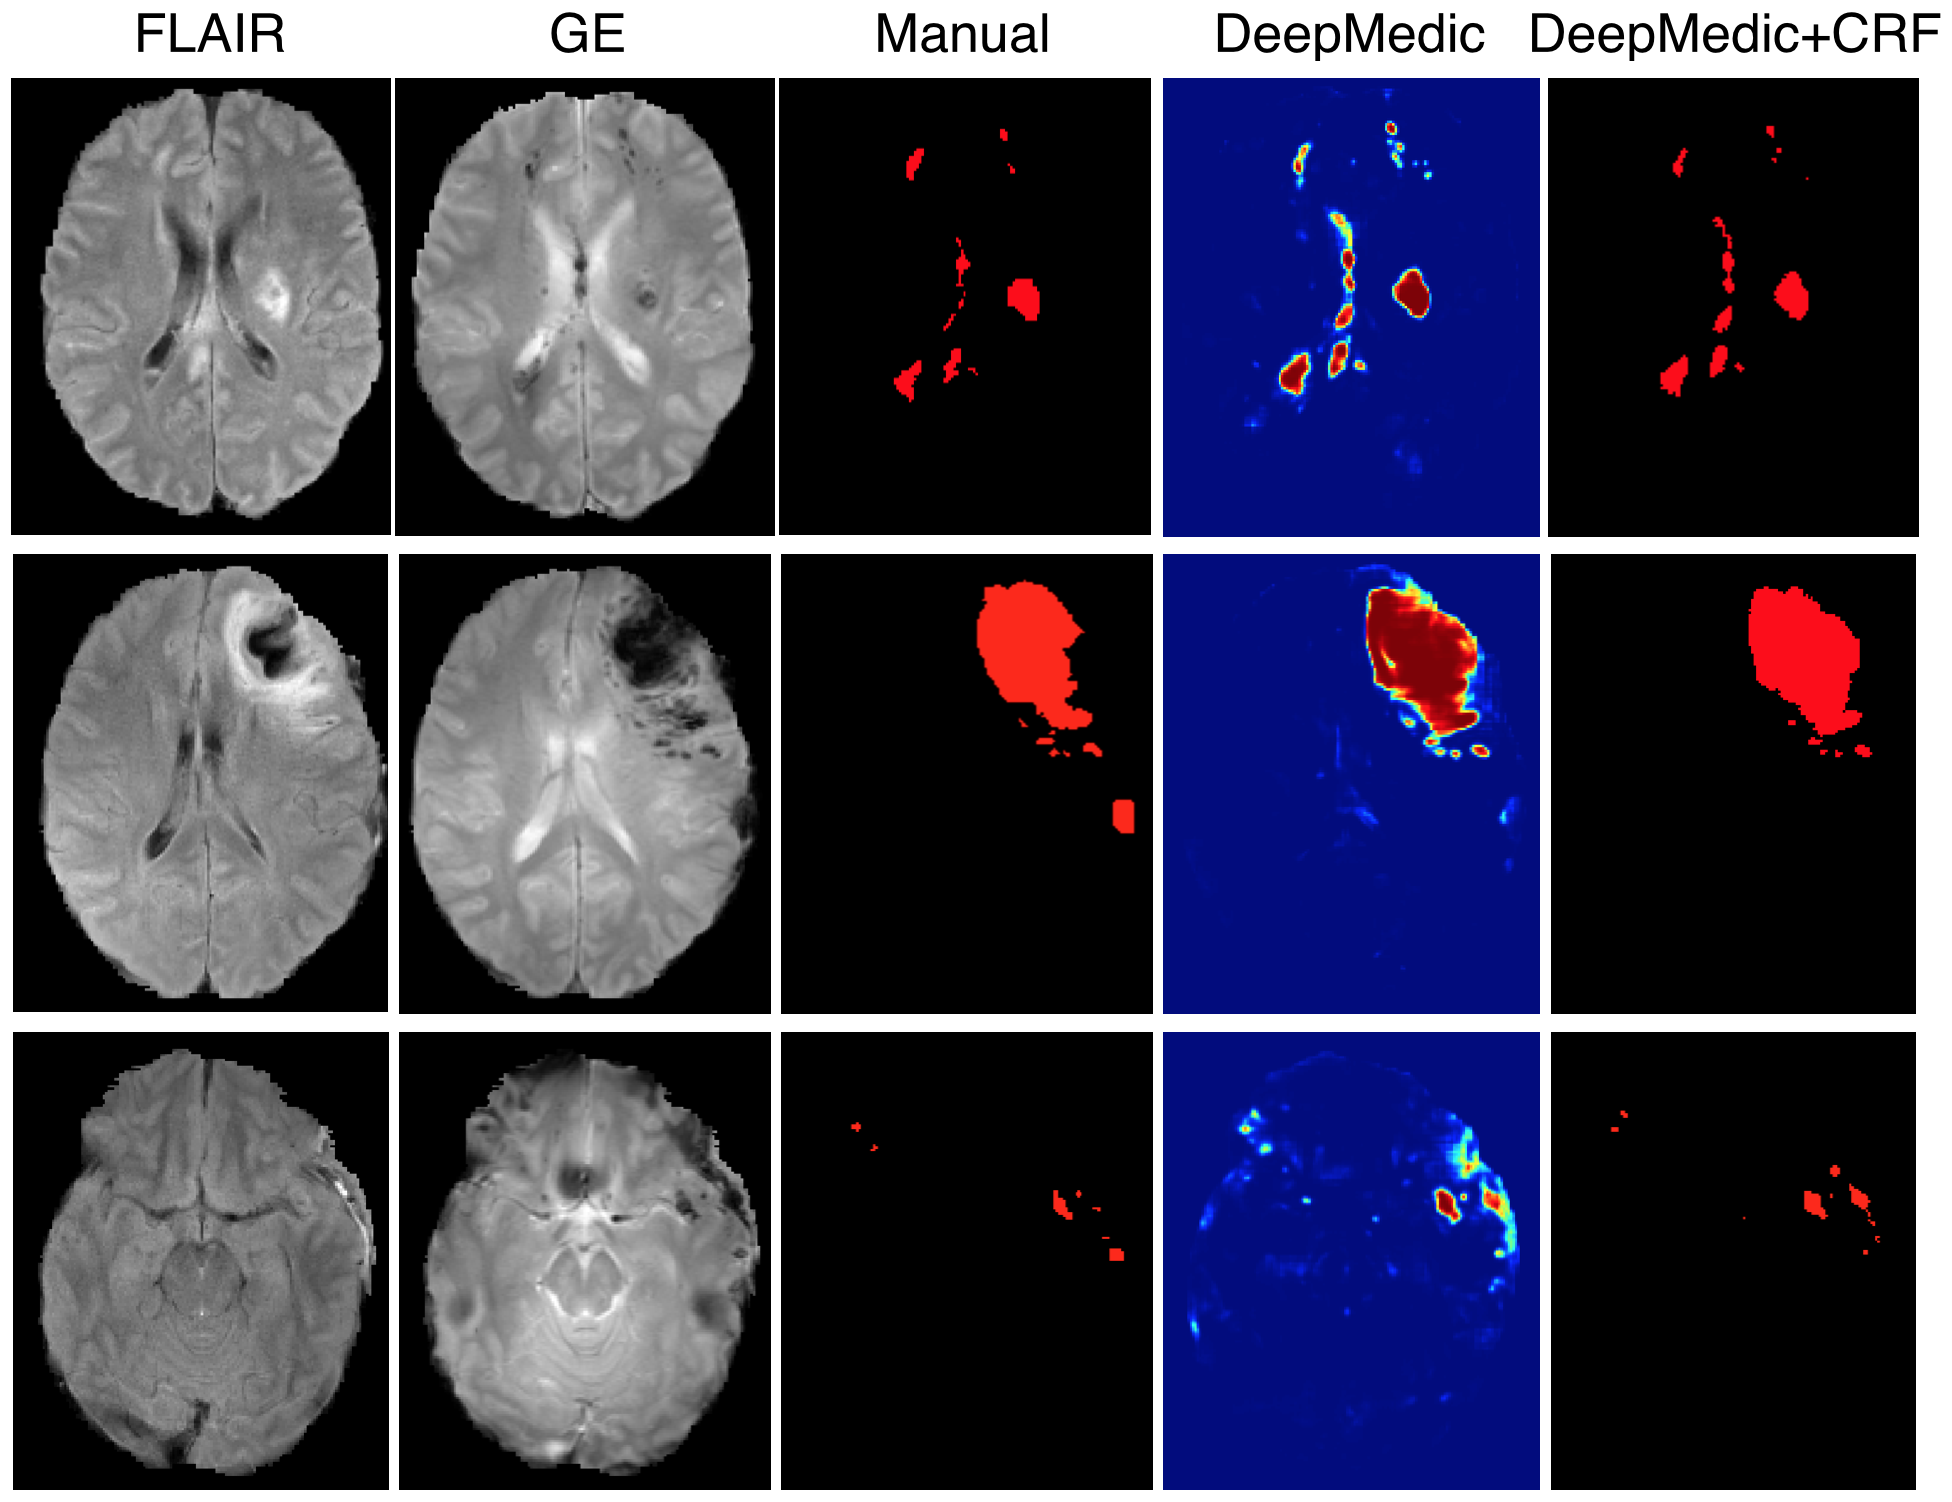
\includegraphics[clip=true, trim=0pt 0pt 0pt 0pt, width=1.0\textwidth]{figures/evaluationSection/tbi/visualsQualitatively/visualsQualitatively4.png}
\end{subfigure}
\vspace{-10pt} %takes away some white space before the caption
\caption{Three examples from the application of our system on the TBI database. It is capable of precise segmentation of both small and large lesions. Second row depicts one of the common mistakes observed. A contusion near the edge of the brain is under-segmented, possibly mistaken for background. Bottom row shows one of the worst cases, representative of the challenges in segmenting TBI. Post-surgical sub-dural debris is mistakenly captured by the brain mask. The network partly segments the abnormality, which is not a celebral lesion of interest.}
\label{fig:evalTbiVisualQuality}
\end{figure}
%\vspace{-1pt} %takes away some white space after figure


\subsection{Brain Tumor Segmentation}
\label{subsec:evalBrats}

\subsubsection{Material and Pre-Processing}

For brain tumors, we evaluate our system on the data from the 2015 Brain Tumor Segmentation Challenge (BRATS) (\cite{Menze2014}). The training set consists of 220 cases with high grade (HG) and 54 cases with low grade (LG) glioma for which corresponding reference segmentations are provided. The segmentations include the following tumor tissue classes: 1) necrotic core, 2) edema, 3) non-enhancing and 4) enhancing core. The test set consists of 110 cases of both HG and LG but the grade is not revealed. Reference segmentations for the test set are hidden and evaluation is carried out via an online system. For evaluation, the four predicted labels are merged into different sets of whole tumor (all four classes), the core (classes 1,3,4), and the enhancing tumor (class 4)\footnote{For interpretation of the results note that, to the best of our knowledge, cases where the \quot{enhancing tumor} class is not present in the manual segmentation are considered as zeros for the calculation of average performance by the evaluation platform, lowering the upper bound for this class.}. For each subject, four MRI sequences are available, FLAIR, T1, T1-contrast and T2. The datasets are pre-processed by the organizers and provided as skull-stripped, registered to a common space and resampled to isotropic $1mm^3$ resolution. Dimensions of each volume are 240$\times$240$\times$155. We add minimal pre-processing of normalizing the brain-tissue intensities of each sequence to have zero-mean and unit variance.


\subsubsection{Experimental Setting}

\textbf{Network configuration and training:} We modify the DeepMedic architecture to handle multi-class problems by extending the classification layer to five feature maps (four tumor classes plus background). The rest of the configuration remains unchanged. We enrich the dataset with sagittal reflections. Opposite to the experiments on TBI, we do not employ the intensity perturbation and dropout on convolutional layers, because the network should not require as much regularisation with this large database. The network is trained on image segments extracted with equal probability centred on the whole tumor and healthy tissue. The distribution of the classes captured by our training scheme is provided in \ref{app:distrTumorClassesTrain}.

To examine our network's behaviour, we first evaluate it on the training data of the challenge. For this, we run a 5-fold cross validation where each fold contains both HG and LG images. We then retrain the network using all training images, before applying it on the test data.

\textbf{CRF configuration:} For the multi-class problem it is challenging to find a global set of parameters for the CRF which can consistently improve the segmentation of all classes. So instead we merge the four predicted probability maps into a single \quot{whole tumor} map for CRF post-processing. The CRF then only refines the boundaries between tumor and background and additionally removes isolated false positives. Similarly to the experiments on TBI, the CRF is configured on a random subset of 44 HG and 18 LG training images, which are then reshuffled into the subsequent 5-fold cross validation. 

\subsubsection{Results}
\label{subsubsec:resBrats2015}



\begin{table}[!h]
\centering
\scriptsize
\caption{Average performance of our system on the training data of BRATS 2015 as computed on the online evaluation platform and comparison to other submissions visible at the time of manuscript submission. Presenting only teams that submitted more than half of the 274 cases. Numbers in bold indicate significant improvement by the CRF, according to a two-sided, paired t-test on the DSC metric (*$p<5\cdot 10^{-2}$, **$p<10^{-3}$). }
\label{table:onlineEvalBrats2015Training}
\begin{tabular}{@{}lllllllllll@{}}
\toprule
              & \multicolumn{3}{c}{DSC}  & \multicolumn{3}{c}{Precision} & \multicolumn{3}{c}{Sensitivity} &       \\ \cmidrule(lr){2-10}
              	& Whole & Core 	& Enh. 		& Whole   & Core  	& Enh.  & Whole & Core & Enh.   	& Cases \\ \midrule
              
Ensemble+CRF		& \textbf{90.1}*	&75.4	& \textbf{72.8}*	& 91.9	& 85.7	& 75.5	& 89.1	& 71.7	& 74.4	&274 \\
Ensemble			& 90.0			&75.5	& 72.8			& 90.3	& 85.5	& 75.4	& 90.4	& 71.9	& 74.3	&274 \\
DeepMedic+CRF	& \textbf{89.8}**&75.0	& \textbf{72.1}*	& 91.5	& 84.4	& 75.9	& 89.1	& 72.1	& 72	.5	&274 \\
DeepMedic		& 89.7			& 75.0	& 72.0			& 89.7	& 84.2	& 75.6	& 90.5	& 72.3	& 72.5	&274 \\

bakas1		 	& 88				& 77		& 68				& 90		& 84		& 68		& 89		& 76		& 75		&186\\
peres1		 	& 87				& 73		& 68				& 89		& 74		& 72		& 86		& 77		& 70		&274\\
anon1		 	& 84				& 67		& 55				& 90		& 76		& 59		& 82		& 68		& 61		&274\\
thirs1		 	& 80				& 66		& 58				& 84		& 71		& 53 	& 79		& 66		& 74		&267\\
peyrj			& 80				& 60		& 57				& 87		& 79		& 59		& 77		& 53		& 60		&274\\
\bottomrule
\end{tabular}
\end{table}

Quantitative results from the application of the DeepMedic, the CRF and an ensemble of three similar networks on the training data are presented in Table \ref{table:onlineEvalBrats2015Training}. The latter two offer an improvement, albeit fairly small since the performance of DeepMedic is already rather high in this task. Also shown are results from previous works, as reported on the online evaluation platform. Various settings may vary among submissions, such as the pre-processing pipeline or the number of folds used for cross-validation. Still it appears that our system performs favourably compared to previous state-of-the-art, including the semi-automatic system of \cite{bakas2015Brats} (bakas1) who won the latest challenge and the method of \cite{pereira2015Brats} (peres1), which is based on grade-specific 2D CNNs and requires visual inspection of the tumor and identification of the grade by the user prior to segmentation. Examples of segmentations obtained with our method are shown in Fig.~\ref{fig:evalBratsVisualQuality}. DeepMedic behaves very well in preserving the hierarchical structure of the tumor, which we account to the large context processed by our multi-scale network.



Table~\ref{table:onlineEvalBrats2015Testing} shows the results of our method on the BRATS test data. Results of other submissions are not accessible. The decrease in performance is possibly due to the the inclusion of test images that vary significantly from the training data, such as cases acquired in clinical centers that did not provide any of the training images, something that was confirmed by the organisers. Note that performance gains obtained with the CRF are larger in this case. This indicates not only that its configuration has not overfitted to the training database but also that the CRF is robust to factors of variation between acquisition sites, which complements nicely the more sensitive CNN.


\begin{table}[!h]
\centering
\scriptsize
\caption{Average performance of our system on the 110 test cases of BRATS 2015, as computed on the online evaluation platform. Numbers in bold indicate significant improvement by the CRF, according to a two-sided, paired t-test on the DSC metric (*$p<5\cdot 10^{-2}$, **$p<10^{-3}$). The decrease of the mean DSC by the CRF and the ensemble for the \quot{Core} class was not found significant.}
\label{table:onlineEvalBrats2015Testing}
\begin{tabular}{@{}llllllllll@{}}
\toprule
              & \multicolumn{3}{c}{DSC}  & \multicolumn{3}{c}{Precision} & \multicolumn{3}{c}{Sensitivity} \\ \cmidrule(l){2-10} 
              & Whole 			& Core & Enh. 			& Whole   & Core   & Enh.	& Whole    & Core   & Enh.   \\ \midrule

DeepMedic     & 83.6  			& 67.4 & 62.9      		& 82.3    & 84.6   & 64.0    & 88.5     & 61.6   & 65.6      \\
DeepMedic+CRF & \textbf{84.7}** 	& 67.0 & 62.9      		& 85.0    & 84.8   & 63.4    & 87.6     & 60.7   & 66.2      \\
Ensemble      & 84.5  			& 66.7 & 63.3      		& 83.3    & 86.1   & 63.2    & 88.9     & 59.9   & 67.3      \\
Ensemble+CRF  & \textbf{84.9}** 	& 66.7 & \textbf{63.4}* 	& 85.3    & 86.1   & 63.4    & 87.7     & 60.0   & 67.4		\\
\bottomrule
\end{tabular}
\end{table}

\begin{figure}[!h]
%\vspace{-1pt} %takes away some white space before figure
\centering
\begin{subfigure}[b]{1.0\textwidth}
	\centering
	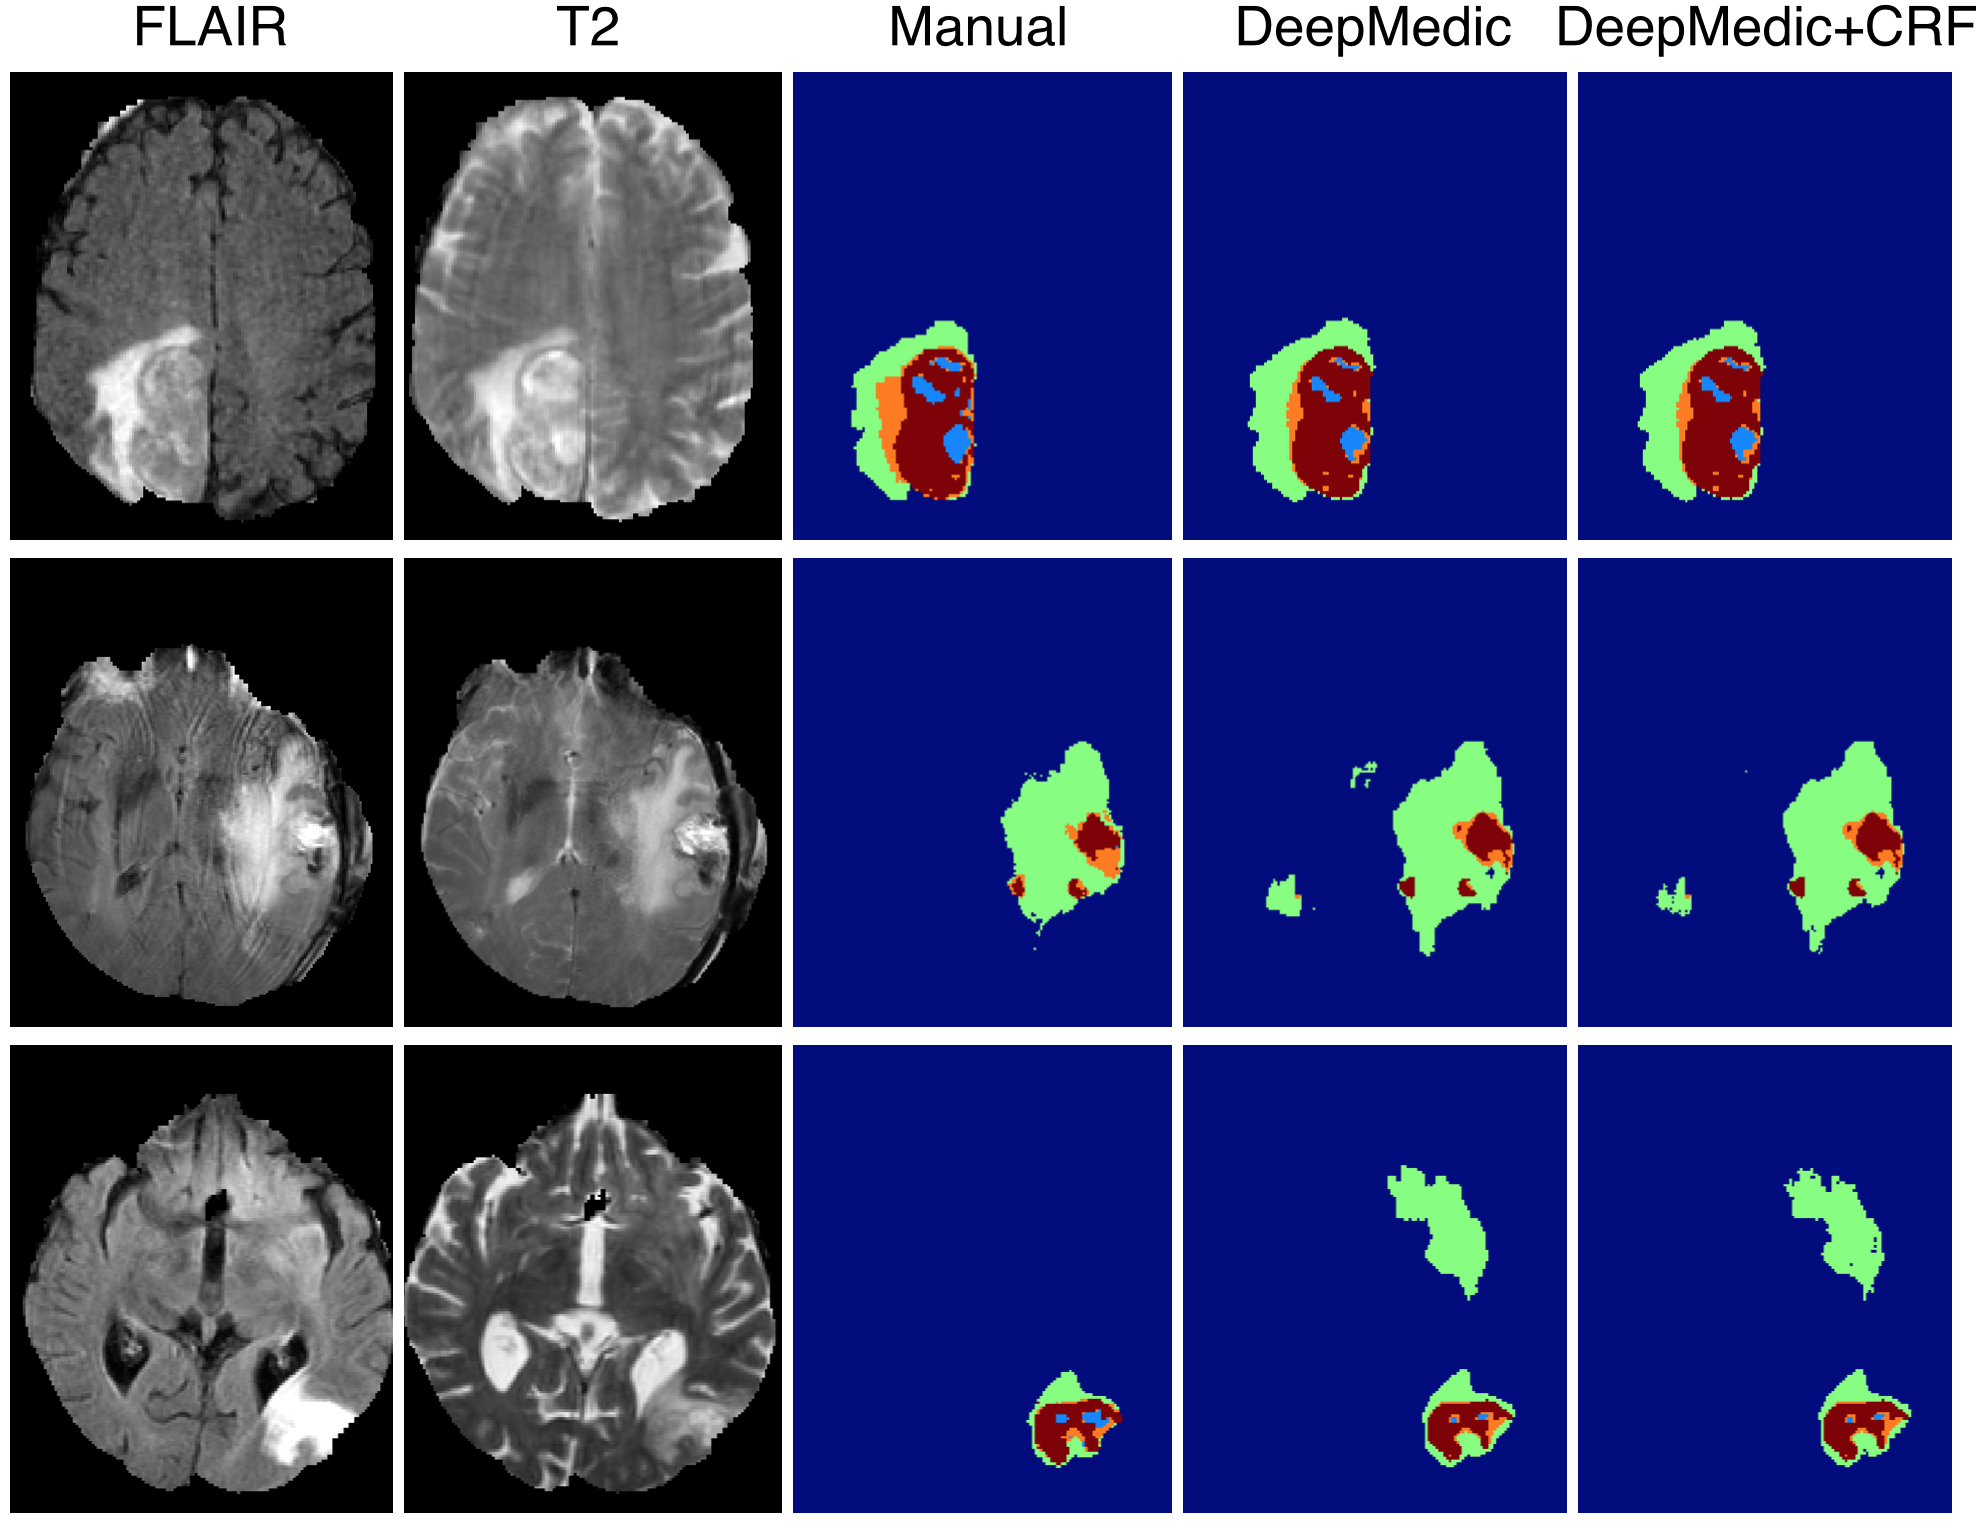
\includegraphics[clip=true, trim=0pt 0pt 0pt 0pt, width=1.0\textwidth]{figures/evaluationSection/brats/qualitative/bratsQualitatively.png}
\end{subfigure}
\vspace{-0pt} %takes away some white space before the caption
\caption{Examples of DeepMedic's segmentation from its evaluation on the training datasets of BRATS 2015. cyan: necrotic core, green: oedema, orange: non-enhancing core, red: enhancing core. (top and middle) Satisfying segmentation of the tumor, regardless motion artefacts in certain sequences. (bottom) One of the worst cases of over-segmentation observed. False segmentation of FLAIR hyper-intensities as oedema constitutes the most common error of DeepMedic.}
\label{fig:evalBratsVisualQuality}
\end{figure}
%\vspace{-1pt} %takes away some white space after figure



\subsection{Ischemic Stroke Lesion Segmentation}
\label{subsec:evalIsles}

\subsubsection{Material and Pre-Processing}

We participated in the 2015 Ischemic Stroke Lesion Segmentation (ISLES) challenge, where our system achieved the best results among all participants on sub-acute ischemic stroke lesions (\cite{maier2017isles}). In the training phase of the challenge, 28 datasets have been made available, along with manual segmentations. Each dataset included T1, T1-contrast, FLAIR and DWI sequences. All images were provided as skull-stripped and resampled to isotropic $1mm^3$ voxel resolution. Each volume is of size 230$\times$230$\times$154. In the testing stage, teams were provided with 36 datasets for evaluation. The test data were acquired in two clinical centers, with one of them being the same that provided all training images. Corresponding expert segmentations were hidden and results had to be submitted to an online evaluation platform. Similar to BRATS, the only pre-processing that we applied is the normalization of each image to the zero-mean and unit variance.

\subsubsection{Experimental Setting}

\textbf{Network Configuration and Training:} The configuration of the network employed is described in \cite{kamnitsas2015Isles}. The main difference with the configuration used for TBI and tumors as employed above is the relatively smaller number of FMs in the low-resolution pathway. This choice should not significantly influence accuracy on the generally small SISS lesions but it allowed us to lower the computational cost.

Similar to the other experiments, we evaluate our network with a 5-fold cross validation on the training datasets. We use data augmentation with sagittal reflections. For the testing phase of the challenge, we trained an ensemble of three networks on all training cases and aggregate their predictions by averaging.

\textbf{CRF configuration:} The parameters of the CRF were configured via a random search on the whole training dataset.

\subsubsection{Results}
\label{subsubsec:resIsles2015}

The performance of our system on the training data is shown in Table~\ref{table:accuracyIslesTraining}. Significant improvement is achieved by the structural regularisation offered by the CRF, although it could be partially accounted for by overfitting the training data during the CRF's configuration. Examples for visual inspection are shown in Fig.~\ref{fig:evalIslesVisualQuality}.

\begin{table}[!h]
\centering
\scriptsize
\caption{Performance of our system on the training data of the ISLES-SISS 2015 competition. Values correspond to the mean (and standard deviation). Numbers in bold indicate significant improvement by the CRF, according to a two-sided, paired t-test on the DSC metric ($p<10^{-2}$).}
\label{table:accuracyIslesTraining}
\begin{tabular}{@{}llllll@{}}
\toprule
\multicolumn{1}{c}{}		& DSC				& Precision		& Sensitivity	& ASSD			& Haussdorf 	\\ \midrule
DeepMedic				& 64(23)		 		& 68(24)			& 65(23)			& 6.99(9.91)		& 73.32(26.03)	\\
DeepMedic+CRF			& \textbf{66(24)}	& 77(24)			& 63(25)			& 5.00(10.33	)	& 55.93(28.55)	\\
\bottomrule
\end{tabular}
\end{table}


\begin{table}[!h]
\centering
\scriptsize
\caption{Our ensemble of three networks, coupled with the fully connected CRF obtained overall best performance among all participants in the testing stage of the ISLES-SISS 2015 challenge. Shown is the performance of our pipeline along with the second and third entries. Values correspond to the mean (and standard deviation).}
\label{table:accuracyIslesTesting}
\begin{tabular}{@{}llllll@{}}
\toprule
\multicolumn{1}{c}{}		& DSC		& Precision		& Sensitivity	& ASSD			& Haussdorf 	\\ \midrule
kamnk1(ours)				& 59(31)		& 68(33)			& 60(27) 		& 7.87(12.63)	& 39.61(30.68)	\\
fengc1					& 55(30)		& 64(31)			& 57(33)	 		& 8.13(15.15)	& 25.02(22.02)	\\
halmh1					& 47(32)		& 47(34)			& 56(33)	 		& 14.61(20.17)	& 46.26(34.81)	\\
\bottomrule
\end{tabular}
\end{table}

For the testing phase of the challenge we formed an ensemble of three networks, coupled with the fully connected CRF. Our submission ranked first, indicating superior performance on this challenging task among 14 submissions. Table~\ref{table:accuracyIslesTesting} shows our results, along with the other two top entries (\cite{feng2015Isles,halme2015Isles}). Among the other participating methods was the CNN of \cite{Havei2015Journal} with 3 layers of 2D convolutions. That method perfomed less well on this challenging task (\cite{maier2017isles}). This points out the advantage offered by 3D context, the large field of view of DeepMedic thanks to multi-scale processing and the representational power of deeper networks. It is important to note the decrease of performance in comparison to the training set. All methods performed worse on the data coming from the second clinical center, including the method of \cite{feng2015Isles} that is not machine-learning based. This highlights a general difficulty with current approaches when applied on multi-center data.

\begin{figure}[!h]
%\vspace{-1pt} %takes away some white space before figure
\centering
\begin{subfigure}[b]{1.0\textwidth}
	\centering
	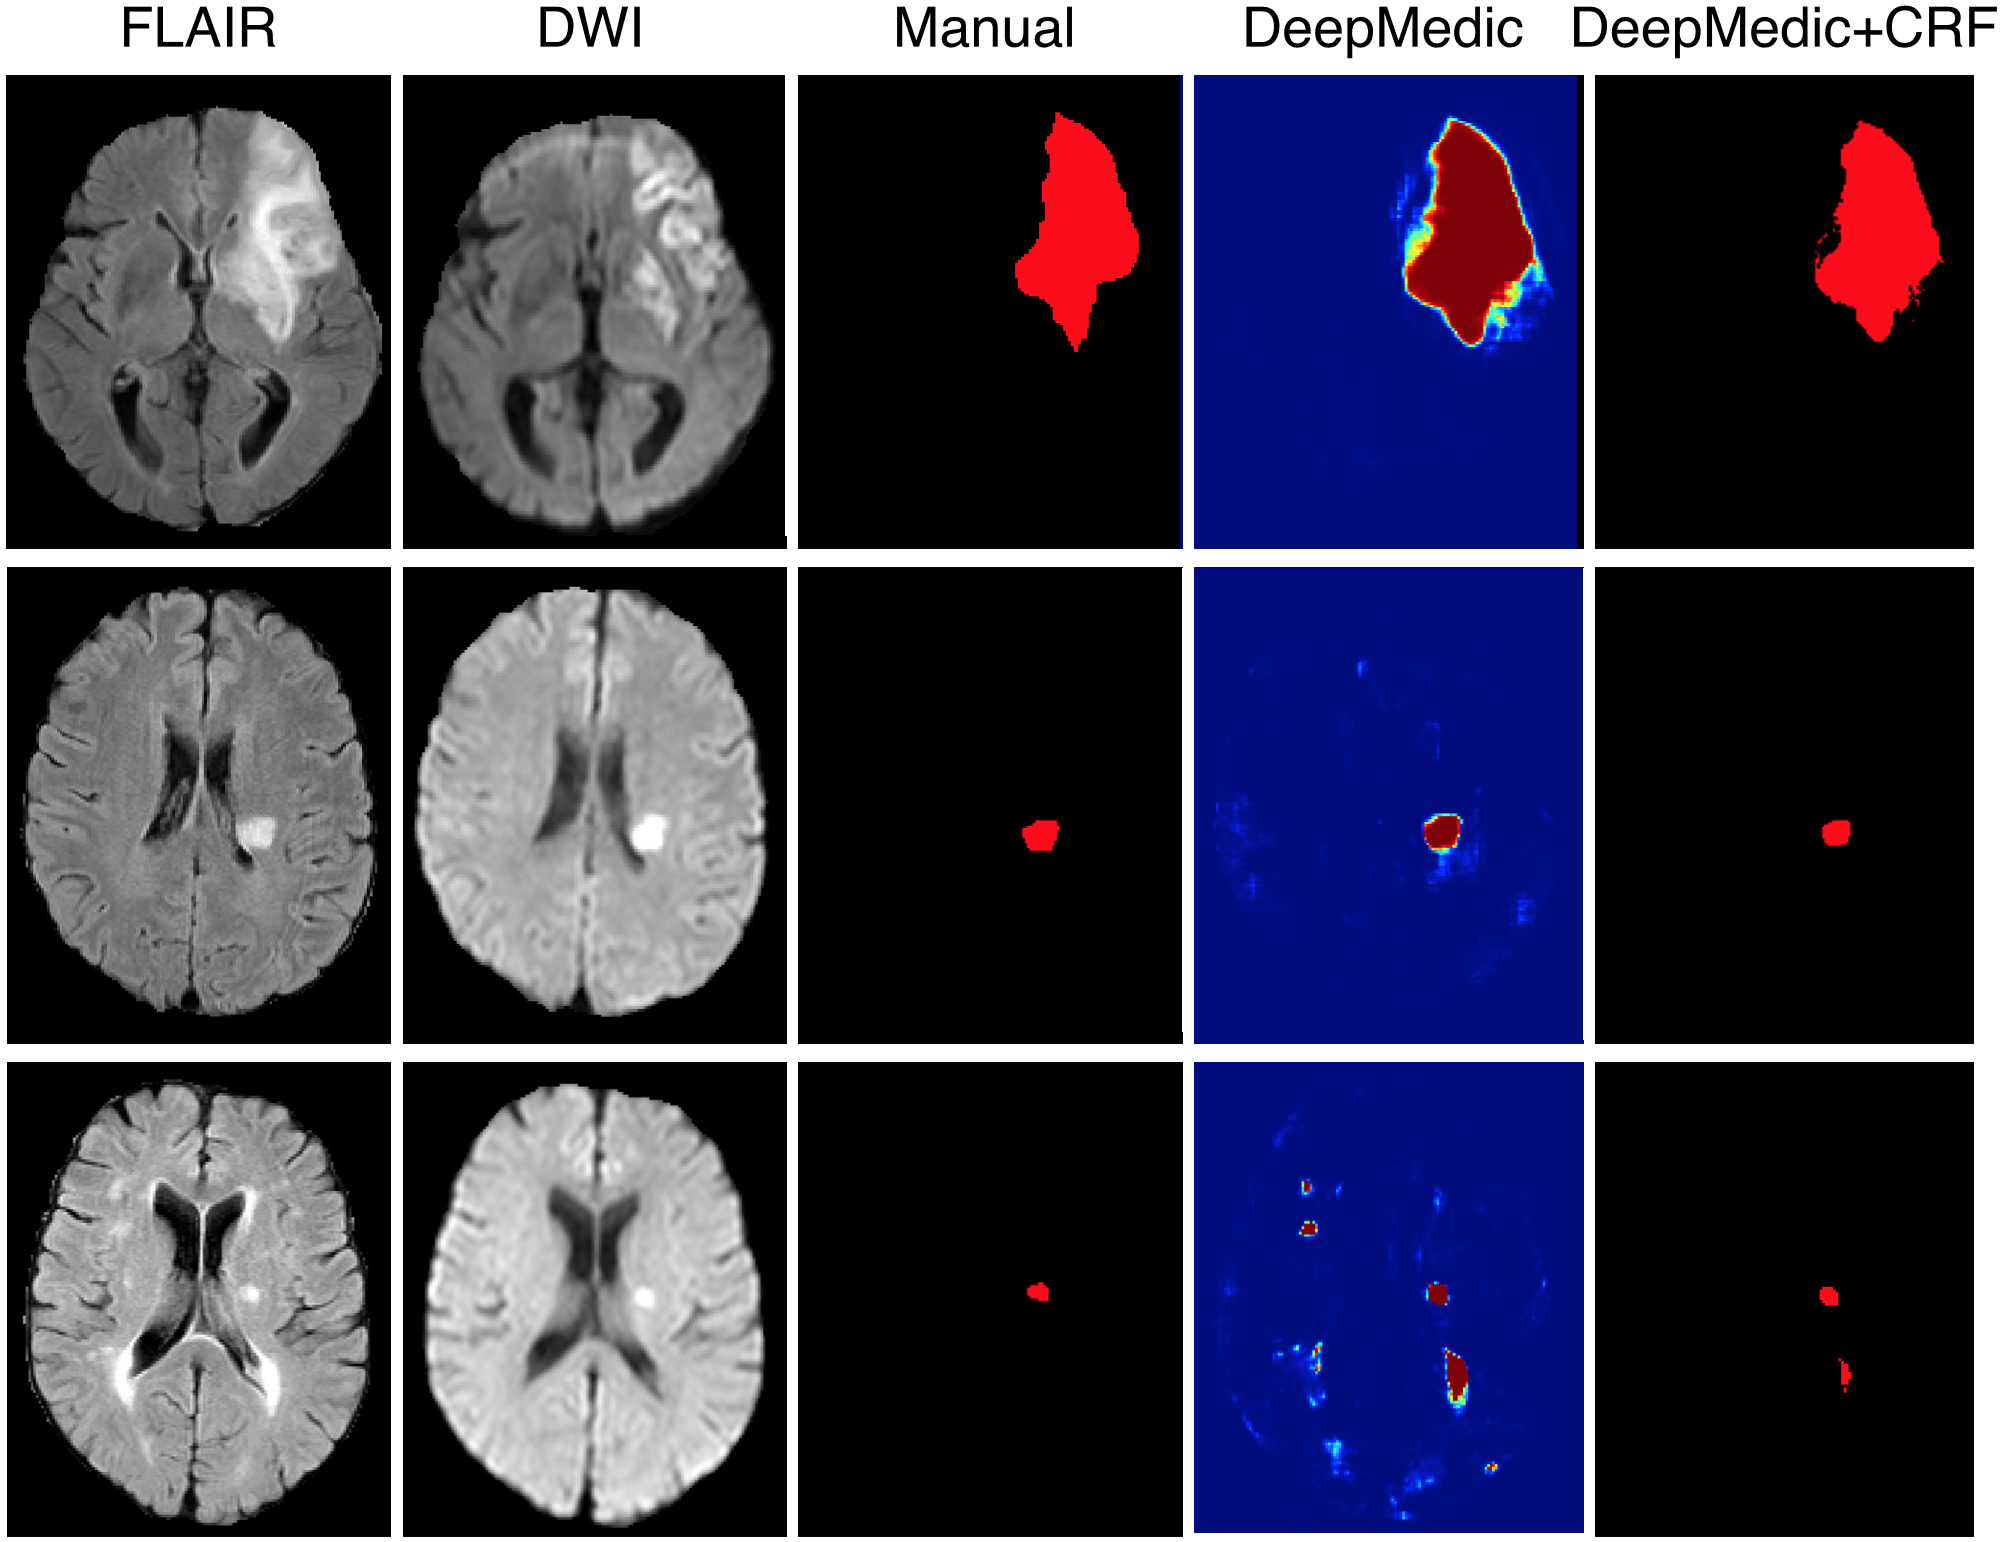
\includegraphics[clip=true, trim=0pt 0pt 0pt 0pt, width=1.0\textwidth]{figures/evaluationSection/isles/qualitative/isles15TrainingQualitatively.png}
\end{subfigure}
\vspace{-0pt} %takes away some white space before the caption
\caption{Examples of segmentations performed by our system on the training datasets of (SISS) ISLES 2015. (top and middle) The system is capable of satisfying segmentation of both large and smaller lesions. (bottom) Common mistakes are performed due to the challenge of differentiating stroke lesions from White Matter lesions. }
\label{fig:evalIslesVisualQuality}
\end{figure}
%\vspace{-1pt} %takes away some white space after figure

\subsection{Implementation Details}
 
Our CNN is implemented using the Theano library (\cite{Bastien-Theano-2012}). Each training session requires approximately one day on an NVIDIA GTX Titan X GPU using cuDNN v5.0. The efficient architecture of DeepMedic also allows models to be trained on GPUs with only 3GB of memory. Note that although dimensions of the volumes in the processed databases do not allow dense training on whole volumes for this size of network, dense inference on a whole volume is still possible, as it requires only a forward-pass and thus less memory. In this fashion segmentation of a volume takes less than 30 seconds but requires 12 GB of GPU memory. Tiling the volume into multiple segments of size $35^3$ allows inference on 3 GB GPUs in less than three minutes.

Our 3D fully connected CRF is implemented by extending the original source code by \cite{Krahenbuhl2013}. A CPU implementation is fast, capable of processing a five-channel brain scan in under three minutes. Further speed-up could be achieved with a GPU implementation, but was not found necessary in the scope of this work.
